\renewcommand{\thechapter}{B}
\chapter{Appendix for Chapter~\ref{chap:ch2}}\label{APP:B}
% \phantomsection\addcontentsline{toc}{chapter}{Appendices}

\renewcommand{\thesection}{B.\arabic{section}}
\renewcommand{\thesubsection}{B.\arabic{section}.\arabic{subsection}}
\renewcommand{\thefigure}{B.\arabic{figure}}
\renewcommand{\thetable}{B.\arabic{table}}
\renewcommand{\theequation}{B.\arabic{equation}}

\section{Theoretical Proofs and Discussions}
% \stoptoc
\subsection[Theoretical Analysis of our Set Function]{Theoretical Analysis of $F(\cdot)$} 
We recall $F(S) \coloneqq \calWF(\bzero)-\min\limits_{\bgamma:\Supp(\bgamma)\subseteq S,\bgamma\geq \bzero} \calWF({\bgamma})=\calWF(\bzero) - \calWF(\bgamma_S)$. Here, $\bgamma_S$ denotes an optimal solution of Eq.~\ref{eqn:uotmmd} with the support specified by the set of tuples $S$.

Now, we first prove that the function $(-\calWF(\cdot))$ has finite restricted strong concavity (RSC) and restricted smoothness (RSM) parameters (Definition~\ref{rsm-rsc}), which will be subsequently used to prove weak submodularity of $F(\cdot)$. With $N=m\times n$, we recall that the restricted domain which we consider is $\Omega_K \coloneqq \{ (\bx, \by)\in \R^N\times \R^N~|~ \bx, \by \geq 0; \|\bx\|_0 \leq K; \|\by\|_0 \leq K\}$, where $K=K_1$ when learning an overall $K$-sparse OT plan and $K=nK_2$ when learning an OT plan with each column $K_2$-sparse. We denote the RSC parameter over $\Omega_K$ as $u_{K}$ and the RSM parameter over $\Omega_K$ as $U_{K}$. An important relation that we use in our work is that when $\hat{K} \leq K$, then $u_{\hat{K}} \geq u_K$ and $U_{\hat{K}} \leq U_K$ which follows by noting that $\Omega_{\hat{K}} \subseteq \Omega_{K}$. 

We also define $\tilde{\Omega}\coloneqq  \{(\bx,\by)\in \R^N\times \R^N~|~ \|\bx-\by\|_0 \leq 1\}$  with the corresponding restricted smoothness parameter $\tilde{U}_1$.

\begin{lemma}\label{lemma:rsc-rsm}
The function $-\calWF$ has a finite restricted strong concavity (RSC) parameter $(u_\Omega)$ and a finite restricted smoothness (RSM) parameter $(U_\Omega)$ over the domain $\Omega$, whenever the employed kernel function $k$ is universal (\citep{SriperumbudurFL11}) and bounded.
\end{lemma}
\begin{proof} We first discuss the case when $\lambda_2=0$ in $\calWF$. Given $\bgamma,\ \bgamma'\in \R^{m\times n}$, we have the following result.
\begin{equation}\label{proof-rsc-rsm}
\begin{array}{l}
-\left(\calWF(\bgamma)  - \calWF(\bgamma')-\langle\nabla \calWF(\bgamma), \bgamma-\bgamma'\rangle\right)\\
\qquad =\lambda_1\left( (\bgamma\bone_n-\bgamma'\bone_n)^\top\bG_{11}(\bgamma\bone_n-\bgamma'\bone_n)+(\bgamma^\top\bone_m-\bgamma'^\top\bone_m)^\top\bG_{22}(\bgamma^\top\bone_m-\bgamma'^\top\bone_m)\right)\\
\qquad =\lambda_1\left( \textup{Tr}\left((\bgamma-\bgamma')^\top \bG_{11} (\bgamma-\bgamma')\bone_n\bone_n^\top\right) + \textup{Tr}\left((\bgamma^\top-\bgamma'^\top)^\top \bG_{22}(\bgamma^\top-\bgamma'^\top)\bone_m\bone_m^\top\right) \right),\vspace{0.4em}
\end{array}
\end{equation}
where $\textup{Tr}(\cdot)$ denotes the trace operator. 

Let $e^1_1$ and $e^2_1$ denote the maximum eigenvalues of $\bG_{11}$ and $\bG_{22}$, respectively. Let $e^1_0$ and $e^2_0$ denote the minimum eigenvalues of $\bG_{11}$ and $\bG_{22}$, respectively. As the Gram matrices are positive semi-definite, these eigenvalues are always non-negative. Further, as the Gram matrices of universal kernels \citep{SriperumbudurFL11} are full-rank \citep[Corollary~32]{Song08}, $e^1_0$ and $e^2_0$ are strictly positive whenever the underlying kernel is universal.

Using the Trace equivalence under cyclic permutation, we have the first term in the RHS of Eq.~\ref{proof-rsc-rsm} as $\textup{Tr}\left(\bG_{11}(\bgamma-\bgamma')\bone_n \left( (\bgamma-\bgamma')\bone_n\right)^\top\right)$. Now, with $\mathbf{v} \coloneqq (\bgamma-\bgamma')\bone_n$, we have the following bound on the first term in the RHS of Eq.~\ref{proof-rsc-rsm}, $e^1_0\textup{Tr}(\mathbf{v}\mathbf{v}^\top \bone_n\bone_n^\top) \leq \textup{Tr}\left(\bG_{11}\mathbf{v}\mathbf{v}^\top\right) \leq e_1^1\textup{Tr}(\mathbf{v}\mathbf{v}^\top \bone_n\bone_n^\top)$. The lower bound simplifies to $e^1_0n \|\bgamma-\bgamma'\|^2$ and the upper bound simplifies to $e_1^1n \|\bgamma-\bgamma'\|^2$.

% TODO: Tr(A^\top A 11^\top)


Similarly, bounding the other term in the RHS of Eq.~\ref{proof-rsc-rsm}, we get that the RSC constant becomes $u_\Omega=\lambda_1(e^1_0n+e^2_0m)$ and the RSM constant becomes $U_\Omega=\lambda_1(e^1_1n + e^2_1m)$. 
With a universal kernel, both $u_\Omega$ and $U_\Omega>0$. Further, with a bounded kernel like the RBF kernel, the maximum eigenvalue of the Gram matrices can be upper-bounded by the maximum row sum (Gershgorin Circle Theorem \citep{gershgorin1931uber}), which is finite for bounded kernels. Thus, we have that $0<u_\Omega \leq U_\Omega<\infty$.

Now, we discuss the case when $\lambda_2>0$. Let $\rm{RHS}_{(\lambda_2=0)}$ denote the RHS in Eq.~\ref{proof-rsc-rsm}. When $\lambda_2>0$, the term $-\left(\calWF(\bgamma)  - \calWF(\bgamma')-\langle\nabla \calWF(\bgamma), \bgamma-\bgamma'\rangle\right) = \rm{RHS}_{(\lambda_2=0)} -\frac{\lambda_2}{2}\|\bgamma-\bgamma'\|^2$. This results in the RSC constant as $\lambda_1(e_0^1n+e_0^2m)+\lambda_2/2$, and the RSM constant as $\lambda_1(e_1^1n+e_1^2m)+\lambda_2/2$, which are again strictly positive and finite under the stated assumption on the kernel function.
\end{proof}

\begin{lemma}\label{lemma2.1}
Let $S\subseteq V$ and $a\in V\setminus S$. Then,
$$F(S\cup \u) - F(S)\geq \frac{1}{2\tilde{U}_1}\left(\max\{-(\nabla \calWF(\bgamma_S))_a,\ 0\}\right)^2,$$
where $\tilde{U}_1$ is the RSM parameter corresponding to $\tilde{\Omega}$.
\end{lemma}
\begin{proof}
We use $\mathbf{g}^+_a(\cdot)\coloneqq \max\{-(\nabla \calWF(\cdot))_a,\ 0\}$.

Let $\bone^{\u}\in \R^{m\times n}$ denote a matrix of zeros with 1 at the index given by $a\in V$. Let $\by^{\u}\coloneqq\bgamma_S+\eta \bone^{\u}$ for some $\eta\geq 0$.
\begin{align*}
F(S\cup \u)-F(S) &= -\calWF(\bgamma_{S\cup \u})+\calWF(\bgamma_S)\\
& \geq -\calWF(\by^{\u}) + \calWF(\bgamma_S)\\
& \geq \langle-\nabla \calWF(\bgamma_S), \eta \bone^{\u} \rangle-\frac{\tilde{U}_1}{2}\eta^2.
\end{align*}
On maximizing wrt $\eta\geq 0,$ we get $F(S\cup \u) - F(S)\geq \frac{1}{2\tilde{U}_1} \left( \mathbf{g}_a^+(\bgamma_S)\right)^2 \ \left(\textup{when }\eta = \frac{\mathbf{g}^+_a(\bgamma_S)}{\tilde{U}_1}\right)$.
\end{proof}

\begin{lemma}\label{lemma2.2}
Let $S,\ A\subseteq V$. Then,
$$F(S\cup A) - F(S)\leq \frac{1}{2u_{\bar{m}}}\sum_{a\in A}\left(\max\{-(\nabla \calWF(\bgamma_S))_a,\ 0\}\right)^2,$$ where $\bar{m} = |S|+|A|$ and $u_{\bar{m}}$ is the RSC parameter corresponding to $\Omega_{\bar{m}}$.
\end{lemma}
\begin{proof}
We use $\mathbf{g}^+_a(\cdot)\coloneqq \max\{-(\nabla \calWF(\cdot))_a,\ 0\}$.

By definition, $\calWF(\bzero)-\calWF(\bgamma_S)= F(S)$ and $\calWF(\bzero)-\calWF(\bgamma_{S\cup A})=F(A\cup S)$. Thus, to upper-bound, $F(S\cup A)-F(S)$, we can upper-bound $\calWF(\bgamma_S)-\calWF(\bgamma_{S\cup A})$. 


Using the RSC and RSM constants of $-\calWF$ (\ref{lemma:rsc-rsm}), we have that,
$$\frac{u_{\bar{m}}}{2}\|\bgamma_{S\cup A}-\bgamma_S\|^2 \leq -\calWF(\bgamma_S) + \calWF(\bgamma_{S\cup A}) + \langle-\nabla \calWF(\bgamma_S), \bgamma_{S\cup A}-\bgamma_S \rangle.$$ On rearranging, we get the following.
\begin{align}\label{lemmaA1.2}
0\leq -\calWF(\bgamma_{S\cup A})+\calWF(\bgamma_S) &\leq \langle -\nabla \calWF(\bgamma_S), \bgamma_{S\cup A}-\bgamma_S \rangle -\frac{u_{\bar{m}}}{2}\|\bgamma_{S\cup A}-\bgamma_S\|^2 \nonumber\\
& \leq \max_{\mathbf{W}:\mathbf{W}\geq \bzero, \mathbf{W}_{V\setminus(S\cup A)}=\bzero} \ \langle-\nabla \calWF(\bgamma_S), \mathbf{W} - \bgamma_S\rangle \nonumber \\ &\qquad\qquad\qquad\qquad\qquad-\frac{u_{\bar{m}}}{2}\|\mathbf{W}-\bgamma_S\|^2.
\end{align} 
The matrix $\mathbf{W}^*$ that attains the maximum can be characterized as follows. 
\newline $\mathbf{W}^*_{S\cup A}=\max\left\{\frac{1}{u_{\bar{m}}}(-(\nabla \calWF(\bgamma_S))_{S\cup A})+(\bgamma_S)_{S\cup A}, \ \bzero \right\}$. Now, from the Karush–Kuhn–Tucker (KKT) conditions, we have that $\forall j\in S$,
$$
(\bgamma_S)_j > 0 \implies -(\nabla \calWF(\bgamma_S))_j=0 \textup{ and }(\bgamma_S)_j = 0 \implies -(\nabla \calWF(\bgamma_S))_j\leq 0.
$$
Hence, $(\mathbf{W}^*-\bgamma_S)_j=0~\forall j\in S$. Also, $(\bgamma_S)_j=0\ \forall j\in A$. Thus, $\forall j\in A, \left(\mathbf{W}^*-\bgamma_S\right)_j=\max \left\{\frac{1}{u_{\bar{m}}}\left(-(\nabla \calWF(\bgamma_S))_j\right), 0 \right\}$. Using this in (\ref{lemmaA1.2}), we get 
$$
F(S\cup A)-F(S)\leq \frac{1}{2u_{\bar{m}}}\sum_{a\in A}\left(\mathbf{g}_a^+(\bgamma_S)\right)^2,
$$ where $\mathbf{g}_a^+(\cdot)\coloneqq \max\{-(\nabla \calWF(\cdot))_a,\ 0\}$ and $\bar{m} = |S|+|A|$.
\end{proof}

\subsection[Proof of Weak-Submodularity of our Set Function]{Proof of Theorem \ref{lemma:subm}}\label{app-lemma:subm}
\lemmasubm*
\begin{proof}
We recall $F(S) \coloneqq \calWF(\bzero)-\min\limits_{\bgamma:\Supp(\bgamma)\in S,~ \bgamma\ge \bzero} \calWF({\bgamma})$. From the definition of $\min$, it follows that $F(\cdot)$ is a monotonically increasing function of $S$, i.e., if $S_1\subseteq S_2\subseteq V$, then $F(S_1)\leq F(S_2)$. As $F(\cdot)$ is monotonically increasing, $F(S)\geq F(\emptyset)=\calWF(\bzero)-\calWF(\bzero)=0$. This shows the non-negativity of $F(\cdot)$. From Lemma \ref{lemma:rsc-rsm}, we know that $(-\calWF(\cdot))$ has a finite RSC and RSM constants. Now, the proof of $\alpha$-weak submodularity of $F(\cdot)$ follows the proof technique used in \citet[Theorem $IV.3$]{gurumoorthy19a}.

For proving weak-submodularity (Sec.~\ref{prelim:subm}), we need to lower bound $F(S\cup \u)-F(S)$ and upper bound $F(S\cup A)-F(S)$. Let $\bar{m}=|S|+|A|$. From Lemma \ref{lemma2.1}, we have that, $F(S\cup \u)-F(S)\geq \frac{1}{2\tilde{U}_1}\left( \bg^+_a(\bgamma_S)\right)^2$. From Lemma \ref{lemma2.2}, we have that, $0\leq F(S\cup A)-F(S)\leq \frac{1}{2u_{\bar{m}}}\sum_{a\in A}\left(\bg^+_a(\bgamma_S) \right)^2.$ Using these, the ratio $\frac{\sum_{a\in A}F(S\cup \u)-F(S)}{F(S\cup A)-F(S)}\geq \frac{u_{\bar{m}}}{\tilde{U}_1}.$ We now lower bound $u_{\bar{m}}$. We recall that $\bar{m}\coloneqq|S|+|A|$ for $S, A\subseteq V$. With the general sparsity constraints on the support (Sec. \ref{gen-sparse}), $\bar{m}\leq 2K_1$, which makes $u_{\bar{m}}\geq u_{2K_1}$ (Sec. \ref{Prel:rsc}). With the column-wise sparsity constraints on the support, (Sec. \ref{subsec:partitionmatroid}), $\bar{m}\leq 2nK_2$, which makes $u_{\bar{m}}\geq u_{2nK_2}$ (Sec. \ref{Prel:rsc}). Hence, we proved that $F(\cdot)$ is $\alpha$-weakly submodularity with $\alpha\geq \frac{u_{2K_1}}{\tilde{U}_1}>0$ for the general sparsity case and $\alpha\geq \frac{u_{2nK_2}}{\tilde{U}_1}>0$ for the column-wise sparsity constraints. Combining the two cases, we have that $\alpha\geq \frac{u_{2K}}{\tilde{U}_1}>0$ where $K$ denotes the sparsity level of the OT plan.
\end{proof}

\subsection[Proof of Approximation Ratio of the Proposed Algorithm for Learning Sparse OT Plans]{Proof of Lemma \ref{lemma:stoch-dash}}\label{app-lemma:stoch-dash}
\lemmastochdash*
\begin{proof}
Let $S^*$ be the optimal support set. We recall that $V$ denote the ground set of cardinality $N= m\times n$ and $K=K_1$ as the general sparsity cardinality constraint. We define $\mathbf{g}^+_j(\bgamma_{S_t})\coloneqq \max\{-(\nabla \calWF(\bgamma_{S_t}))_j,\ 0\}$.

Let the randomly chosen set $R_t$ consist of $s=\frac{N}{K}\log{\frac{1}{\zeta}}$ elements from $V\setminus S_{t-1}$. We first estimate the probability that $R_t\cap (S^*\setminus S_{t-1})$ is non-empty.

\begin{align}
\Pr\left[R_t\cap (S^*\setminus {S_{t-1}})\neq\emptyset\right] & = 1-\Pr\left[R_t\cap (S^*\setminus {S_{t-1}})=\emptyset\right] \nonumber\\
& = 1-\left(1-\frac{|S^*\setminus {S_{t-1}}|}{|V\setminus {S_{t-1}}|} \right)^s \nonumber\\
& \geq 1-e^{-s\frac{|S^*\setminus {S_{t-1}}|}{|V\setminus {S_{t-1}}|}} \ (\because 1-x\leq e^{-x}) \nonumber\\
& \geq 1-e^{-s\frac{|S^*\setminus {S_{t-1}}|}{N}} \ (\because |V\setminus {S_{t-1}}|\leq N) \nonumber\\
& \stackrel{(1)}{\geq} \left(1-e^{\frac{sK}{N}}\right)\frac{|S^*\setminus {S_{t-1}}|}{K} \ \tag{Using concavity of $f(x)=1-e^{-\frac{s}{N}x}$} \nonumber\\
& = (1-\zeta)\frac{|S^*\setminus {S_{t-1}}|}{K}\label{app:stoch0}
\end{align}
The inequality (1) is detailed as follows. As $f(x) = 1-e^{-\frac{s}{N}x}$ is a concave function for $x\in \R$ and as $\frac{|S^*\setminus {S_{t-1}}|}{K}\in [0, 1]$, we have that $f\left(\frac{|S^*\setminus {S_{t-1}}|}{K} K+ \left(1-\frac{|S^*\setminus {S_{t-1}}|}{K}\right)\cdot 0\right)\geq \frac{|S^*\setminus {S_{t-1}}|}{K} f(K) + \left(1-\frac{|S^*\setminus {S_{t-1}}|}{K}\right)f(0)$.

Now, we observe that, for an element $a$ to be picked by Algorithm \ref{alg:stoch-dash}, $\mathbf{g}^+_a(\bgamma_{S_{t-1}})\geq \mathbf{g}^+_b(\bgamma_{S_{t-1}}),\ \forall b\in R_t\cap \left(S^*\setminus S_{t-1}\right)$ (if non-empty). Thus, we have that,
\begin{align}
\mathbf{g}^+_a(\bgamma_{S_{t-1}})\geq \mathbf{g}^+_b(\bgamma_{S_{t-1}}) &\implies \left(\mathbf{g}^+_a(\bgamma_{S_{t-1}})\right)^2 
\geq \left(\mathbf{g}^+_b(\bgamma_{S_{t-1}})\right)^2 \nonumber
\end{align}
\begin{equation}\label{app:stoch1}
    \implies \E\left[\left(\mathbf{g}^+_a(\bgamma_{S_{t-1}})\right)^2|S_{t-1}\right] \geq \E\left[\left(\mathbf{g}^+_b(\bgamma_{S_{t-1}})\right)^2|S_{t-1}\right] \Pr\left[ R_t\cap \left(S^*\setminus S_{t-1}\right)\neq \emptyset \right],
\end{equation}
for any element $b\in R_t\cap \left(S^*\setminus S_{t-1}\right)$ (if non-empty).

We then use that $R_t$ is equally likely to contain each element of $S^*\setminus S_{t-1}$, so a uniformly random element of $R_t\cap \left(S^*\setminus S_{t-1}\right)$ is a uniformly random element of $S^*\setminus S_{t-1}$. From (\ref{app:stoch1}), 
\begin{align}\label{app:stoch2}
\E\left[\left(\mathbf{g}^+_a(\bgamma_{S_{t-1}})\right)^2|S_{t-1}\right] & \geq \Pr\left[ R_t\cap \left(S^*\setminus S_{t-1}\right)\neq \emptyset \right]\frac{1}{|S^*\setminus S_{t-1}|}\sum_{b\in S^*\setminus S_{t-1}}\left(\mathbf{g}^+_b(\bgamma_{S_{t-1}})\right)^2\nonumber\\
& \geq \frac{1-\zeta}{K} \sum_{b\in S^*\setminus S_{t-1}}\left(\mathbf{g}^+_b(\bgamma_{S_{t-1}})\right)^2,
\end{align}
where the last inequality uses inequality~\ref{app:stoch0}.
Using $(S_{t+1}= S_t\cup \u)$ in the above relation and Lemma \ref{lemma2.1} we get,
\begin{equation}\label{app:stoch3}
\E\left[2\tilde{U}_1\left(F(S_{t+1})- F(S_t)\right)|S_t\right]\geq \E\left[ \left(\mathbf{g}^+_a(\bgamma_{S_t}) \right)^2|S_t \right].
\end{equation}
Also, from Lemma \ref{lemma2.2}, we have that,
\begin{equation}\label{app:stoch4}
\frac{1-\zeta}{K}\sum_{b\in S^*\setminus S_t} \left( \mathbf{g}^+_b(\bgamma_{S_t}) \right)^2\geq \frac{2u_{\bar{m}}(1-\zeta)}{K} \left( F(S^*)-F(S_t)\right)\geq \frac{2u_{2K}(1-\zeta)}{K} \left( F(S^*)-F(S_t)\right),
\end{equation}
where the last inequality uses that $\bar{m} = |S_t| + |S^*\setminus S_t|\leq 2K$ and hence $u_{\bar{m}} \geq u_{2K}$.

From inequalities \ref{app:stoch2}, \ref{app:stoch3},  and \ref{app:stoch4}, we get the following.
\begin{align*}
& \E\left[2\tilde{U}_1\left(F(S_{t+1})- F(S_t)\right)|S_t\right] \geq \frac{2u_{2K}(1-\zeta)}{K} \left( F(S^*)-F(S_t)\right)\\
\implies & \E\left[\left(F(S_{t+1})- F(S_t)\right)|S_t\right] \geq \frac{u_{2K}(1-\zeta)}{K\tilde{U}_1} \left( F(S^*)-F(S_t)\right) \\
\implies & \E\left[F(S_{t+1})- F(S_t)\right] \geq \frac{u_{2K}(1-\zeta)}{K\tilde{U}_1} \left( F(S^*)-\E\left[F(S_t)\right]\right) \ \tag{Taking an expectation over $S_t$}
\end{align*}
On re-arranging and using induction, we get
\begin{align*}
\E\left[F(S_K)\right]&\geq \frac{u_{2K}(1-\zeta)}{K\tilde{U}_1} F(S^*)\left( \sum_{t=0}^{K-1} \left( 1-\frac{u_{2K}(1-\zeta)}{K\tilde{U}_1} \right)^t \right)\\
    &\stackrel{(2)}{\geq} \left(1-\left( 1-\frac{u_{2K}(1-\zeta)}{K\tilde{U}_1} \right)^K \right)F(S^*)  \\
    & \geq \left(1-e^{-\frac{u_{2K}(1-\zeta)}{\tilde{U}_1}} \right)F(S^*) \ \tag{Using $e^{-x}\geq 1-x$} \\
    & = \left(1-e^{-r(1-\zeta)} \right)F(S^*) \ \tag{where $r=\frac{u_{2K}}{\tilde{U}_1}$}
    \\
    & \stackrel{(3)}{\geq} \left(1-e^{-r}-\zeta\right)F(S^*).
\end{align*}
The inequality (2) uses that $\frac{u_{2K}}{\tilde{U}_1}\in (0, 1)$ and then applies the sum of geometric series formula. We have already discussed the non-negativity of this term. We now discuss how $\frac{u_{2K}}{\tilde{U}_1}\leq 1$.
Using Lemma~\ref{lemma2.2} with $A=\{a\}$ and combining the result with Lemma~\ref{lemma2.1} where $S=S_K$ in both the Lemma's, we get that $\frac{u_{K+1}}{\tilde{U}_1}\leq 1$. As $2K\geq K+1,\ u_{2K}\leq u_{K+1} \ \implies \frac{u_{2K}}{\tilde{U}_1}\leq 1$.
% Now, as the RSC parameter derived in the proof of Lemma~\ref{lemma:rsc-rsm} is a function of the minimum eigenvalues of the Gram matrices, it is independent of the sparsity level ($K$) of the transport plan and hence $\frac{u_{K+1}}{\tilde{U}_1}=\frac{u_{2K}}{\tilde{U}_1}\leq 1$.

The inequality (3) is detailed as follows. Let us first consider a function $f$ over the domain $[0,  1]$ defined as $f(x) = z^x-xz$ for some $z\geq 0$. This is a convex function with $f(0)=1, f(1)=0$. Thus, $z^x-xz\leq 1$. Taking $z=e^r$ proves the result. The proof technique is inspired by the proof for the stochastic-greedy algorithm \citep{mirzasoleiman15a}.
\end{proof}

\subsection[Proof of Approximation Ratio of the Proposed Algorithm for Learning Column-wise Sparse OT Plans]{Proof of Lemma \ref{lemma:struc-dash}}\label{app-lemma:struc-dash}
In this subsection, we use $K$ to denote the overall cardinality constraint of the column-wise sparse transport plan, i.e., $K=nK_2$.
Our proof is inspired by the approximation ratio proof in \citet{pmlr-v80-chen18b}.  We first discuss the following lemma where our proof differs from that in \citet{pmlr-v80-chen18b}.

Let $OPT$ be an arbitrary optimal solution. As $F(\cdot)$ is monotone, we may assume $OPT$ is a base of $\calM$. \citet[Lemma 2.2]{pmlr-v80-chen18b} describes constructing a random set $OPT_t$ for which $S_t\cup OPT_t$ is a base, for every $0\leq t \leq K$. Using these, we present the crucial lemma as follows.
\begin{lemma}\label{matroid} For every $1\leq t \leq K, ~ \E[F(S_t)]\geq \E[F(S_{t-1})]+\alpha \frac{\E[F(OPT_{t-1}\cup S_{t-1})]-\E[F(S_{t-1})]}{K-t+1}$, where $\alpha=\frac{u_{2K}}{\tilde{U}_1}$.
\end{lemma}
\begin{proof}
The base $OPT_{t-1}$ is a possible candidate to be the maximizing base, $M_t$ at iteration $t$. Now, with the criteria used in Algorithm \ref{alg:colsparseOT_dash} to pick the next element, we have the following.
\begin{align}
\sum_{a\in M_t}\mathbf{g}^+(a|S_{t-1}) \geq \sum_{a\in OPT_{t-1}} \mathbf{g}^+(a|S_{t-1}) \implies \sum_{a\in M_t}\left(\mathbf{g}^+(a|S_{t-1})\right)^2 & \geq \sum_{a\in OPT_{t-1}} \left(\mathbf{g}^+(a|S_{t-1})\right)^2.\nonumber
\end{align}
Now, using Lemma \ref{lemma2.1} and Lemma \ref{lemma2.2}, we have that, $$\sum_{a\in M_t} 2\tilde{U}_1 F(a|S_{t-1})\geq 2u_{\bar{m}} F(OPT_{t-1}|S_{t-1})\implies \sum_{a\in M_t} F(a|S_{t-1})\geq \frac{u_{\bar{m}}}{\tilde{U}_1} F(OPT_{t-1}|S_{t-1}),$$
where $\bar{m} = |OPT_{t-1}| + |S_{t-1}|$.

We denote $\frac{u_{2K}}{\tilde{U}_1}(\leq \frac{u_{\bar{m}}}{\tilde{U}_1})$ by $\alpha$. Algorithm \ref{alg:colsparseOT_dash} adds a uniformly random element $a\in M_t$ to the set $S_{t-1}$ to obtain the set $S_t$. As $M_t$ is of the size $K-t+1$,
\begin{align*}
\E[F(S_t)]  = F(S_{t-1}) + \E[F(a|S_{t-1})]  & = F(S_{t-1}) + \frac{1}{K-t+1} \sum_{a\in M_t}F(a|S_{t-1})\\
& \stackrel{(1)}{\geq} F(S_{t-1}) + \frac{\alpha}{K-t+1}F(OPT_{t-1}|S_{t-1})\\ & = F(S_{t-1}) + \alpha\frac{F(OPT_{t-1}\cup S_{t-1})-F(S_{t-1})}{K-t+1},
\end{align*}
where inequality (1) uses that $F(\cdot)$ is $\alpha$-weakly submodular.
\end{proof}

\noindent We now give the proof sketch of Lemma \ref{lemma:struc-dash}.
\lemmastrucdash*
\begin{proof}
From \citet[Lemma 2.3]{pmlr-v80-chen18b}, $\E[F(OPT_t)]\geq \left[ 1-\left( \frac{t+1}{K+1}\right)^{\alpha}\right] F(OPT)$ for $1\leq t \leq K$. This result uses the non-negativity of $F(\cdot)$ and the property that $OPT_t$ is a uniformly random subset (of size $K-t$) of $OPT$.

Combining this result with Lemma \ref{matroid}, \citet[Corollary 2.5]{pmlr-v80-chen18b} gives us that for every $1\leq t\leq K, ~ \E[F(S_t)]\geq \E[F(S_{t-1})] + \alpha \frac{\{1-[t/(K+1)]^\alpha\}F(OPT)-\E[F(S_{t-1})]}{K-t+1}$. This sets up for an induction, and the rest of the proof for the approximation ratio exactly follows the induction-based proof in \citet[Theorem 2.6]{pmlr-v80-chen18b}.
\end{proof}

\subsection[Deriving the Dual of our Column-wise Sparse OT Problem]{Proofs of Lemma \ref{lemma:dual} and Proposition \ref{prop:dualitygap}}\label{app:dual}
We discuss the proof of Lemma \ref{lemma:dual} together with the proof of Proposition \ref{prop:dualitygap} after restating these claims.
\lemmadual*
\propdualitygap*
\begin{proof}
We begin by re-stating the primal problem.
\begin{equation}
    \begin{array}{l}
        \min\limits_{\bgamma\geq \bzero} P(\bgamma)\big(\coloneqq \langle\mathbf{C},\bgamma\rangle + \sum_{j=1}^n \Theta(\bgamma_j)
        + \lambda_1(\|\bgamma\bone-\bmu\|_{\bG_{11}}^2+\|\bgamma^\top\bone-\bnu\|_{\bG_{22}}^2)\big),\label{app:primal}
    \end{array}
\end{equation}
where $\Theta(\bgamma_j)=\frac{\lambda_2}{2}\|\bgamma_j\|^2 + \delta_{B_{K_2}}(\bgamma_j)$ and $B_{K_2} = \{\bz\in \R_{+}^m:\|\bz\|_0\leq K_2\}$.
We use auxiliary variables $\mathbf{p}\in\R^m$ and $\mathbf{q}\in\R^n$ to set $\bgamma\bone-\bmu=\mathbf{p}$ and $\bgamma^\top\bone-\bnu=\mathbf{q}$. The Lagrangian becomes
\begin{align*}
    \min\limits_{\bgamma\geq \bzero; \mathbf{p}\in \R^m; \mathbf{q} \in \R^n} \ \langle\mathbf{C},\bgamma\rangle + \sum_{j=1}^n \Theta(\bgamma_j) + \lambda_1(\|\mathbf{p}\|_{\bG_{11}}^2+\|\mathbf{q}\|_{\bG_{22}}^2) &+ \balpha^\top(\mathbf{p}-\bgamma \bone + \bmu) \\
    &+ \bbeta^\top(\mathbf{q}-\bgamma^\top \bone + \bnu),
\end{align*}
where $\balpha\in \R^m$ and $\bbeta \in \R^n$. We simplify the Lagrangian as follows.
\begin{align*}
    \min\limits_{\bgamma\geq \bzero; \mathbf{p}\in \R^m; \mathbf{q} \in \R^n} \ \langle\mathbf{C},\bgamma\rangle + \sum_{j=1}^n \Theta(\bgamma_j) + \lambda_1(\|\mathbf{p}\|_{\bG_{11}}^2+\|\mathbf{q}\|_{\bG_{22}}^2) &  +  \balpha^\top(\mathbf{p}-\bgamma \bone + \bmu) 
    \\ & + \bbeta^\top(\mathbf{q}-\bgamma^\top \bone + \bnu)
\end{align*}
This further simplifies as follows.
\begin{align*}
    \sum_{j=1}^n \min\limits_{\bgamma_j\geq \bzero} \Big(\langle\mathbf{C}_j-\balpha -\bbeta_j\bone , \bgamma_j\rangle +  \Theta(\bgamma_j) \Big) + \min\limits_{\mathbf{p}\in \R^m; \mathbf{q} \in \R^n}\Big( \lambda_1(\|\mathbf{p}\|_{\bG_{11}}^2+\|\mathbf{q}\|_{\bG_{22}}^2) & + \balpha^\top(\mathbf{p} + \bmu) \\ 
    & + \bbeta^\top(\mathbf{q} + \bnu)\Big)
\end{align*}
\begin{align}
    =& \sum_{j=1}^n - \Theta^*(\balpha + \bbeta_j\bone -\bC_j) + \min\limits_{\mathbf{p}\in \R^m; \mathbf{q} \in \R^n}\Big(\lambda_1(\|\mathbf{p}\|_{\bG_{11}}^2+\|\mathbf{q}\|_{\bG_{22}}^2) + \balpha^\top(\mathbf{p} + \bmu) + \bbeta^\top(\mathbf{q} + \bnu)\Big).\label{lag}
\end{align}
From the optimality conditions, we have that $2\lambda_1\bG_{11}\mathbf{p}+\balpha = 0$ and $2\lambda_1\bG_{22}+\bbeta=0$. On substituting the values of $\mathbf{p}$ as $\bgamma\bone -\bmu$ and $\mathbf{q}$ as $\bgamma^\top \bone -\bnu$, we get the solutions as $\balpha_S=2\lambda_1\bG_{11}(\bmu-\bgamma\bone)$ and $\bbeta_S = 2\lambda_1\bG_{22}(\bnu-\bgamma^\top \bone)$ proving Proposition \ref{prop:dualitygap}. 

Using this relationship in equation (\ref{lag}), the simplified Lagrangian is denoted by $D(\balpha,\bbeta)$. The dual problem of (\ref{app:primal}) then becomes the following.
\begin{align*}
     \max\limits_{\balpha\in\R^m,\bbeta\in\R^n} D(\balpha,\bbeta)
     =\max\limits_{\balpha\in\R^m,\bbeta\in\R^n} \langle\balpha,\bmu\rangle + \langle\bbeta,\bnu\rangle &- \frac{1}{4\lambda_1}\balpha^\top \bG_{11}^{-1}\balpha
         -\frac{1}{4\lambda_1} \bbeta^\top \bG_{22}^{-1}\bbeta\\
         & -\sum_{j=1}^n \Theta^*(\balpha+\bbeta_j\bone - \bC_j).
\end{align*}
This proves Lemma \ref{lemma:dual}.
\end{proof}

\subsection{Classical Algorithms for Submodular Maximization\\ under Matroid Constraints}
We present the classical algorithms for maximization of (weakly) submodular functions subject to matroid constraints. Algorithm~\ref{alg:gensparseOT_greedy} and Algorithm~\ref{alg:gensparseOT_dash} correspond to the Uniform Matroid constraints, and Algorithm~\ref{alg:matroid} corresponds to the Partition Matroid constraints.
\begin{algorithm}[ht!]
\caption{Classical greedy algorithm for learning sparse transport plans}\label{alg:gensparseOT_greedy}
\begin{algorithmic}[1]
\Require $\lambda_1, \lambda_2, \bmu, \bnu, \bC, \bG_{11}, \bG_{22}$, sparsity level $K_1$.
\State $S_0=\emptyset, \bgamma_{S_0}=\bzero$.
\For{$t=1,\ldots,K_1$}
\State  $a \in \argmax_{e\in V\setminus S_{t-1}}(F(S_{t-1}\cup \{e\})-F(S_{t-1}))$ (ties broken arbitrarily)
\State $S_t = S_{t-1}\cup \u$
\EndFor
\State $\bgamma_{S_{K_1}} = \argmin_{\bgamma:\Supp(\bgamma)\in S_{K_1},~ \bgamma\ge \bzero}{\calWF(\bgamma)}$
\State \textbf{return} $S_{K_1}, \bgamma_{S_{K_1}}$
\end{algorithmic}
\end{algorithm}

\begin{algorithm}[ht!]
\caption{Gradient-based greedy algorithm for learning sparse transport plans}\label{alg:gensparseOT_dash}
\begin{algorithmic}[1]
\Require  $\lambda_1, \lambda_2, \bmu, \bnu, \bC, \bG_{11}, \bG_{22}$, sparsity level $K_1$.
\State $S_0=\emptyset, \bgamma_{S_0}=\bzero$ and $\bg = -\nabla \calWF(\bgamma_{S_0})$.
\For{$t=1,\ldots,K_1$}
\State $a \in \argmax_{e\in V\setminus S_{t-1}}{\mathbf{g}_e}$ (ties broken arbitrarily)
\State  $S_t = S_{t-1}\cup \u$
\State  $\bgamma_{S_t} = \argmin_{\bgamma:\Supp(\bgamma)\in S_t,~ \bgamma\ge \bzero}{\calWF(\bgamma)}$
\State $\mathbf{g} = -\nabla \calWF(\bgamma_{S_t})$
\EndFor
\State \textbf{return} $S_{K_1}, \bgamma_{S_{K_1}}$
\end{algorithmic}
\end{algorithm}

\begin{algorithm}[ht!]
\caption{Classical randomized residual greedy algorithm for learning column-wise sparse transport plans}\label{alg:matroid}
\begin{algorithmic}[1]
\Require  $\lambda_1, \lambda_2, \bmu, \bnu, \bC, \bG_{11}, \bG_{22}$, per column sparsity level $K_2$.
\State $S_0=\emptyset, \bgamma_{S_0} = \bzero, K=nK_2,\mathbf{g} = -\nabla \calWF(\bgamma_{S_0})$.
\For{$t=1,\ldots,K$}
\State $M_t\leftarrow $ a maximal independent set of $\calM_2/S_{t-1}$ maximizing $\sum_{a\in M_t}F(a|S_{t-1})$ (ties broken arbitrarily)
\State $a\leftarrow$ a uniformly random element from $M_t$
\State $S_t = S_{t-1}\cup \u$
\State $\bgamma_{S_t} = \argmin_{\bgamma:\Supp(\bgamma)\in S_t,\bgamma\ge \bzero}{\calWF(\bgamma)}$ 
\State $\mathbf{g} = -\nabla \calWF(\bgamma_{S_{t}})$

\EndFor
\State \textbf{return} $S_{K}, \bgamma_{S_{K}}$
\end{algorithmic}
\end{algorithm}

\resumetoc

\section{More on Experiments}\label{app:exp}
\stoptoc
We present details of experiments discussed in the chapter, along with some additional results.

\paragraph{Common Experimental Details:} In the proposed approach, we either use the RBF kernel $k(x, y) = \exp{\frac{-\|x-y\|^2}{2\sigma^2}}$ or kernels from the inverse multiquadratic (IMQ) family: $k(x, y) = (\sigma^2+\|x-y\|^2)^{-0.5}$ (\citep{dwivedi2022generalized}; referred to as IMQ) and $k(x, y) = \left(\frac{1+\|x-y\|^2}{\sigma^2}\right)^{-0.5}$ (\citep{cadgan}; referred to as IMQ-v2). 
% These are the universal kernels \citep{SriperumbudurFL11, NIPS2017_dfd7468a, cadgan, dwivedi2022generalized, mmd-uot, cot}. 
The cost function is squared-Euclidean unless otherwise mentioned. We also normalize the cost matrix such that all entries are upper-bounded by 1. The coefficient of quadratic regularization $\lambda_2$ is 0 unless otherwise mentioned.

The experiments in $\S$ \ref{colsparseexp} are done on an NVIDIA A100-SXM4-40GB GPU, and the remaining experiments are done on an NVIDIA GeForce RTX 4090 GPU.

\begin{figure}[ht]
    \centering
    \begin{tabular}{ccc}
        \subcaptionbox{}{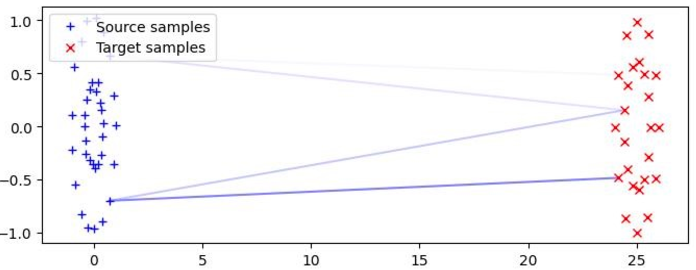
\includegraphics[width=0.32\textwidth]{chapter-2/images/1.pdf}} & 
        \subcaptionbox{}{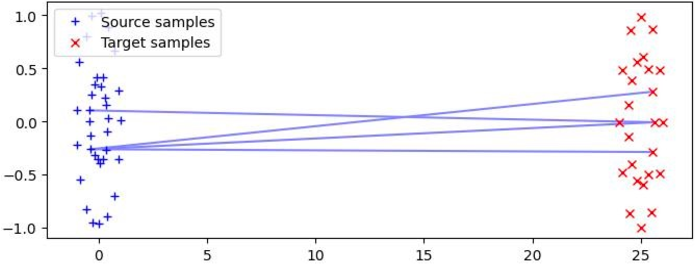
\includegraphics[width=0.32\textwidth]{chapter-2/images/2.pdf}} &
        \subcaptionbox{}{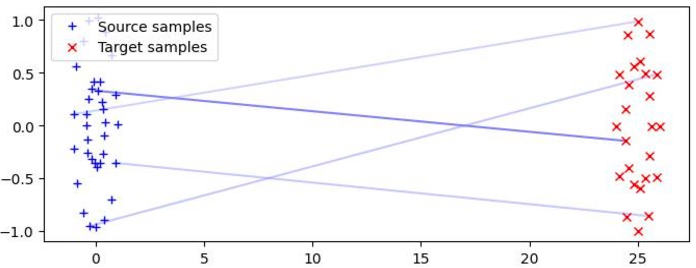
\includegraphics[width=0.32\textwidth]{chapter-2/images/3.pdf}}
    \end{tabular}
\caption{(Best viewed in color.) 
The source samples are shown in blue, and the target samples are shown in red. We show an edge between source point $i$ and target point $j$ if $\bgamma_{i, j}>0$. The intensity of the color represents the magnitude of $\bgamma_{i, j}$. (a) SSOT \citep{blondel18a} results in 4 non-zero entries in $\bgamma$. (b) The top-3 entries of the MMD-OT transport plan. (c) General-SparseOT plan with $K_1=4$. We can see that the support points of the transport plan obtained by General-SparseOT are the most diverse, resulting in one-to-one mapping between the source and the target.}
\label{synthF1}
% \vskip -0.2in
\end{figure}

\begin{figure}[ht]
    \centering
    \begin{tabular}{ccc}
        \subcaptionbox{}{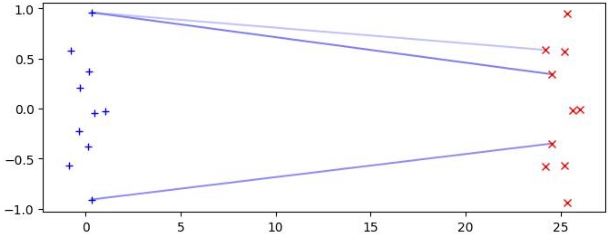
\includegraphics[width=0.32\textwidth]{chapter-2/images/10_1.pdf}} & 
        \subcaptionbox{}{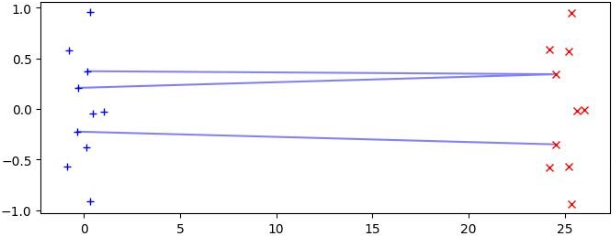
\includegraphics[width=0.32\textwidth]{chapter-2/images/10_2.pdf}} &
        \subcaptionbox{}{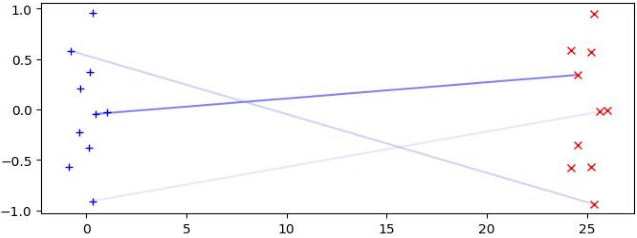
\includegraphics[width=0.32\textwidth]{chapter-2/images/10_3.pdf}}
    \end{tabular}
    \caption{(Best viewed in color.) 
The source samples are shown in blue, and the target samples are shown in red. We show an edge between source point $i$ and target point $j$ if $\bgamma_{i, j}>0$. The intensity of the color represents the magnitude of $\bgamma_{i, j}$. (a) SSOT \citep{blondel18a} results in 3 non-zero entries in $\bgamma$. (b) The top-3 entries of the MMD-OT transport plan. (c) General-SparseOT plan with $K_1=3$. We can see that the support points of the transport plan obtained by General-SparseOT are the most diverse, resulting in one-to-one mapping between the source and the target.}
\label{synthF1-10}
\end{figure}


\subsection{Diversity in the Chosen Support} 
\paragraph{Experimental Setup and Results.}
Our Algorithm for the General-SparseOT problem iteratively builds a support set where a support point $(i, j)$ that maximally results in a strictly positive marginal gain is added to the support set. Thus, we expect points in the support set to be diverse. Such diverse solution sets for submodular maximization have also been observed in \cite{DasKempe18}. Diversity in the support set of a transport plan implies primarily learning one-to-one mappings between the source and the target points rather than one-to-many or many-to-one mappings. 

We show the results with two different sets of source and target data. In Figure~\ref{synthF1}, we observe the diversity in the learned transport plan with $K=4$ on the two-dimensional source and target sets. 
Figure~\ref{synthF1}(a) shows the transport plan obtained using SSOT \citep{blondel18a}, which ends up with 4 support points. We then compute the OT plan with MMD-OT thresholded to keep the 4 coupling values having the largest magnitude. Finally, we compare these with the solution of General-SparseOT obtained with sparsity level $K_1=4$. We can see that the General-SparseOT plan exhibits diversity and doesn't end up with many-to-one couplings like SSOT and MMD-OT. The same pattern was observed for another set of source and target data points shown in Figure~\ref{synthF1-10}.

\paragraph{Validation Details.}
The details of the hyperparameters used for Fig. \ref{synthF1} are as follows. We consider empirical measures over the two-dimensional source and target samples with no. of source samples as 35 and no. of target samples as 25. The coefficient of regularization hyperparameter for SSOT is chosen from \{0.1, 0.5, 1\}. The result in Fig. \ref{synthF1}(a) has a coefficient of 0.5, which resulted in the OT plan with the most diverse support points. The results obtained with the proposed method and with MMD-OT use RBF kernel with $\sigma^2$ as $1$ and $\lambda_1$ as 10. Fig. \ref{synthF1-10} shows results with empirical measures over the two-dimensional source and target samples with no. of source and target samples as 10 each. The coefficient of regularization for SSOT is 0.5, which resulted in the OT plan with the most diverse support points. The results obtained with the proposed method and with MMD-OT use IMQ kernel with $\sigma^2$ as $10$ and $\lambda_1$ as 10.

\subsection{Gradient Flow} 
\paragraph{Experimental Setup and Results.}
The gradient flow experiment deals with transforming an initial (source) distribution $\bmu$ into a target distribution $\bnu$ by taking gradient steps, governed by a learning rate proportional to $-\nabla_{(\bmu)_t}\textup{D}((\bmu)_t, (\bnu)_t)$ at each timestep $t$, where $\textup{D}$ is a divergence over measures.
Prior works have employed an OT-based divergence \citep{fatras2019learnwass, bomb-ot} and used the Euler scheme for solving this problem \citep{FeydySVATP19}. Often, in practice, the gradient updates are performed only over the support of the distribution, keeping the mass values of the distribution fixed to uniform \citep{bomb-ot}. 

In our experiment, the initial source distribution and the target distributions are shown in Figure~\ref{grad-flow}(a). Both the source and the target sets have $1000$ data points each. The learning rate for gradient updates is fixed to $0.01$, and the number of iterations is set to $2450$. 
Figures~\ref{grad-flow}(b)~\&~\ref{grad-flow}(c) plot the results for MMD-OT and the proposed General-SparseOT formulations (solved with Algorithm \ref{alg:gensparseOT_dash}), respectively. We observe that the transformed source distribution obtained by General-SparseOT closely mimics the target distribution, while the solution obtained with MMD-OT performs poorly. This is interesting because while General-SparseOT employs an MMD-OT-based objective, the additional sparsity constraint and the submodular maximization approach ensure that the support for General-SparseOT is diversely selected. This seems to make the gradients with the proposed approach more informative and aid in better convergence.
\paragraph{Validation Details.}
The details of hyperparameters used for Fig. \ref{grad-flow} are as follows. For the proposed method, we use IMQ kernel with $\sigma^2$ as $10^{-4}$ and $\lambda_1$ as $10^{-1}$. For MMD-OT, we also use the IMQ kernel but additionally validated over a range of hyperparameters: $\sigma^2\in\{10^{-4}, 10^{-3}, 10^{-2}\},~ \lambda_1\in \{10^{-4}, 10^{-3}, 10^{-2}, 10^{-1}, 1, 10\}$. The best $\sigma^2$ is $10^{-3}$ and the best $\lambda_1= 10^{-2}$.

\begin{figure*}
% \vskip 0.2in
\centering{
% \begin{center}
    \begin{tabular}{ccc}
        \subcaptionbox{}{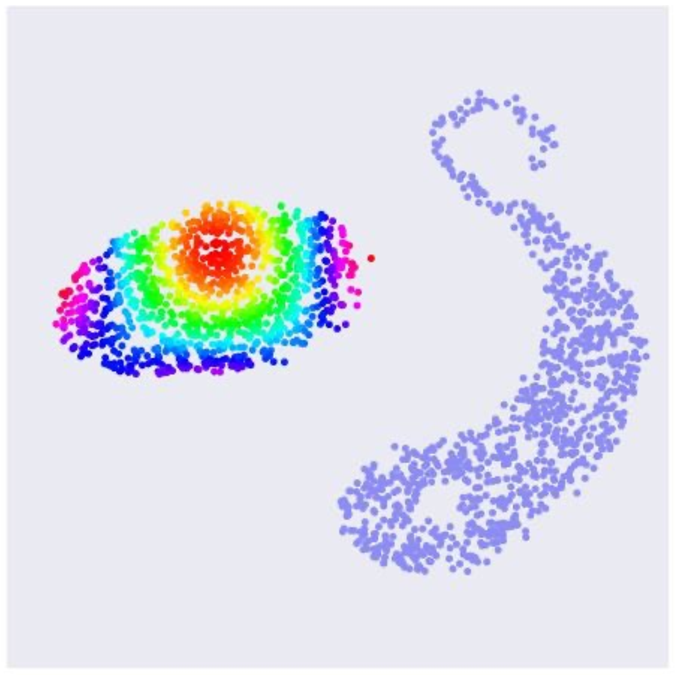
\includegraphics[width=0.32\textwidth]{chapter-2/images/gradient-flow/GF1.pdf}} & 
        \subcaptionbox{}{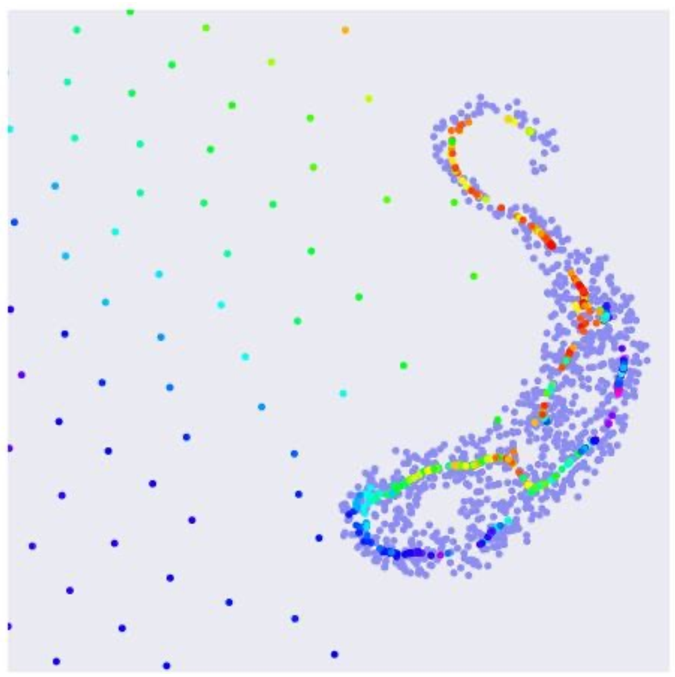
\includegraphics[width=0.32\textwidth]{chapter-2/images/gradient-flow/GF2.pdf}} & 
        \subcaptionbox{}{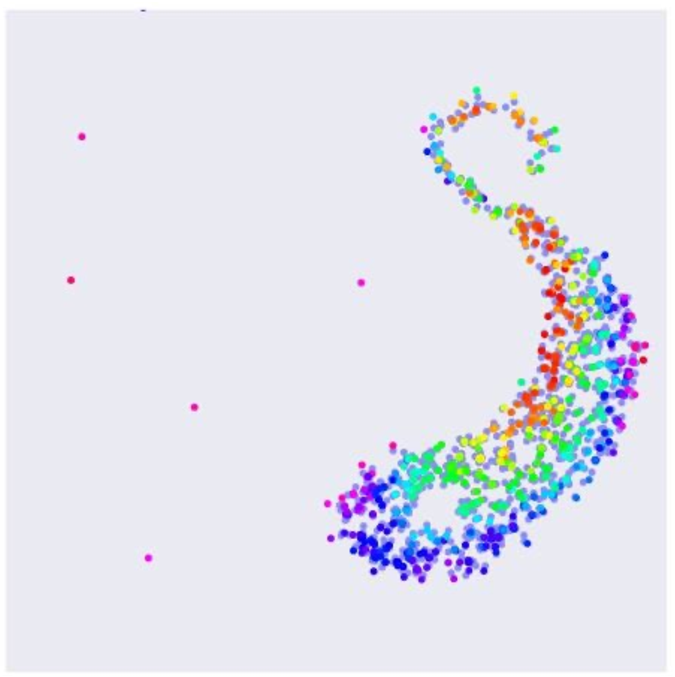
\includegraphics[width=0.32\textwidth]{chapter-2/images/gradient-flow/GF3.pdf}} \\
    \end{tabular}
 \caption[Results on the gradient flow experiment.]{(Best viewed in color.) (a) Initial source points (rainbow color) on the left and target points (in blue) on the right. (b) Gradient Flow results of MMD-OT (c) Gradient Flow results of proposed General-SparseOT.}
\label{grad-flow}
% \end{center}
}
% \vskip -0.2in
\end{figure*}
 
\subsection{Designing Topology} \label{app:spfd}
Table \ref{app-table-top} shows the detailed result where we present the mean and the standard deviation of expected profit when run with different seeds for data generation. We also show the result with our non-stochastic Algorithm \ref{alg:gensparseOT_dash}.
\paragraph{Validation Details.} The validation set is generated following the procedure given by \citet{ijcai2023p679}. Both the GSOT's hyperparameters ($\alpha$ and $\rho$) are independently chosen from the set $\{10^{-2}, 10^{-1}, 1, 10\}$. For the proposed approach, the regularization parameter $\lambda_1$ and the kernel parameter $\sigma^2$ are chosen from the sets $\{1, 10, 100\}$ and $\{10^{-3}, 10^{-2}, 10^{-1}, 1\}$, respectively.

The hyperparameters chosen after validation are as follows. The proposed approach uses RBF kernel with $\sigma^2 =1$ and $\lambda_1=100$. The hyperparameters $(\alpha, \rho)$ in GSOT are set as $(10, 1)$. 
\paragraph{Computation Time.} Table \ref{table: Time T1} compares the computation time of the GSOT method and the proposed approach. This computation time includes the time taken to compute the OT plans and the time taken to compute the overall profit as described in $\S$ \ref{gensparseexp}. The algorithm to compute the overall profit is the same for both methods. We observe that the proposed approach not only outperforms quantitatively but is also faster than the GSOT baseline.


\begin{table}[t]
\caption{Expected profit (higher is better) for SPFD experiment with varying network size constraint $l$. Proposed refers to our General-SparseOT formulation (\ref{eqn:gensparse}). We report the mean and std. deviation with 5 different seed values. We observe that our approach outperforms GSOT.}
\label{app-table-top}
% \vskip 0.15in
% \setlength{\tabcolsep}{4pt}
\centering
\begin{tabular}{lccc}
\toprule
Method & $l=100$ & $l=175$ & $l=250$\\
\midrule
    GSOT \citep{ijcai2023p679} & $0.014 \pm 0.001$ & $0.031 \pm 0.001$ & $0.044 \pm 0.002$ \\
    \rowcolor{green!10}
    Proposed (Algorithm \ref{alg:gensparseOT_dash}) & $0.152 \pm 0.006$ & $0.212 \pm 0.011$ & $0.252\pm0.008$\\
    \rowcolor{green!10}
    Proposed (Algorithm \ref{alg:stoch-dash}, $\zeta= 10^{-2}$)  & $0.166 \pm 0.013$ & $ 0.224 \pm 0.029 $ & $ \mathbf{0.293\pm0.023}$\\
    \rowcolor{green!10}
    Proposed (Algorithm \ref{alg:stoch-dash}, $\zeta= 10^{-3}$) & $ \mathbf{0.167\pm0.017}$ & $ 0.238 \pm 0.021$ & $0.286 \pm 0.017$\\
    \rowcolor{green!10}
    Proposed (Algorithm \ref{alg:stoch-dash}, $\zeta= 10^{-4}$) & $0.147 \pm 0.018$ & $ \mathbf{0.240\pm0.015}$ & $ 0.274 \pm 0.008$\\
\bottomrule
\end{tabular}
% \vskip -0.1in
\end{table}
 \begin{table}
\caption{Computation time (s) for results in Table \ref{table-top}.}
\label{table: Time T1}
% \vskip 0.15in
\centering
\setlength{\tabcolsep}{4pt}
\begin{tabular}{lccc}
\toprule
Method & $l=100$ & $l=175$ & $l=250$\\
\midrule
    GSOT \citep{ijcai2023p679} & 17.69 & 20.09 & 23.00 \\
    Proposed ($\zeta= 10^{-2}$) & 6.74 & 11.99 & 17.59 \\
    Proposed ($\zeta= 10^{-3}$) & 6.33 & 12.03 & 17.93 \\
    Proposed ($\zeta= 10^{-4}$) & 6.44 & 11.92 & 17.68 \\
\bottomrule
\end{tabular}
% \vskip -0.1in
\end{table}

\subsection{Monolingual Word Alignment}\label{app:word_alignment}
We detail the $\rm{F}_1$ scores reported in Table \ref{table-word}, with the associated precision and recall values in Table \ref{table-waln2}. 

\paragraph{Validation Details.} The Wiki dataset consists of 2514 training instances, 533 validation instances, and 1052 test instances. The validation data split is the same provided by \citet{arase-etal-2023-unbalanced}. For the baseline methods, the results are obtained by running the code along with optimal hyperparameters shared by \citet{arase-etal-2023-unbalanced}. We detail the grid for choosing hyperparameters by referring to the baselines used by \cite{arase-etal-2023-unbalanced} as BOT (balanced OT), POT (partial OT), entropy regularized KL-regularized OT ($\epsilon$-KLOT). We also compare with MMD-OT \citep{mmd-uot} and SSOT \citep{blondel18a}. The grid for choosing hyperparameters for BOT, POT and $\epsilon$-KLOT are as follows \cite{arase-etal-2023-unbalanced}, i.e., the regularization hyperparameters for BOT, POT have 50 equally-spaced values between 0 and 1, and the regularization hyperparameter for $\epsilon$-KLOT has 200 equally spaced values in the log space between -3 and 3. For SSOT, the regularization hyperparameter $\lambda$ is chosen from $\{10^{-7}, 10^{-6}, \ldots, 1\}$. 
For both MMD-OT and the proposed approach: (a) the kernel function is chosen from RBF and IMQ, (b) the kernel hyperparameters are tuned from the set $\{m/8, m/4, m, 4m, 8m\}$, where $m$ denotes the median used in median heuristics \citep{gretton12a}, and (c) $\lambda_1$ is tuned from the set $\{0.1, 1, 10\}$. For the proposed method, $\lambda_2$ is validated on the set $\{0.1,0\}$.

The chosen hyperparameters for SSOT and MMD-OT and the proposed approach are as follows. The coefficient of $\ell_2$-norm regularization $\lambda$ for SSOT is $10^{-4}$. 
For MMD-OT, IMQ kernel is chosen with $\sigma^2=4m$ and $\lambda_1$ as 10. 
For our approach, the chosen kernel is RBF with $\sigma^2=m/8$, $\lambda_1=1$, and $\lambda_2=0.1$. 

\paragraph{Computation Time.} The average time (in seconds) to compute OT plans is listed as follows. (a) BOT, POT, and $\epsilon$-KLOT baselines of \citet{arase-etal-2023-unbalanced} require 0.01 seconds, (b) SSOT requires 0.08 seconds, (c) MMD-OT requires 0.40 seconds, and (d) our approach requires 1.06 seconds. 

\begin{table}[t]
\caption{Precision and Recall values on the test split of the Wiki dataset. Higher values are better.}
\label{table-waln2}
% \vskip 0.15in
% \begin{center}
\centering{
\begin{tabular}{lcccc}
\toprule
\multirow{2}{*}{Method} & \multicolumn{2}{c}{Null Alignments} & \multicolumn{2}{c}{Overall}\\
 &  Precision & Recall & Precision & Recall\\
\midrule
    Balanced OT \cite{arase-etal-2023-unbalanced} & \textbf{79.80} &	{80.29} & {95.11} &	\textbf{94.81} \\
    Partial OT \cite{arase-etal-2023-unbalanced} & 66.96 &	79.01  & 93.64 &	94.67\\
    $\epsilon$-KLOT \cite{arase-etal-2023-unbalanced} & 77.31 &	80.16 &	 94.50 &	{94.75} \\
    MMD-OT \cite{mmd-uot} & 76.41 & 75.42 & 92.73 &	93.57 \\
    SSOT \cite{blondel18a} & 23.02 &	40.64  & 57.71 & 72.15 \\
    \rowcolor{green!10}
    Proposed & {79.14}	& \textbf{80.72} &	 \textbf{95.13} &	94.45 \\
\bottomrule
\end{tabular}
}
% \end{center}
% \vskip -0.1in
\end{table}

\subsection{Learning Sparse-Mixture-of-Experts}\label{colsp}

% \begin{figure}[ht]
%     \centering
%     \begin{tabular}{cc}
%         \subcaptionbox{...}{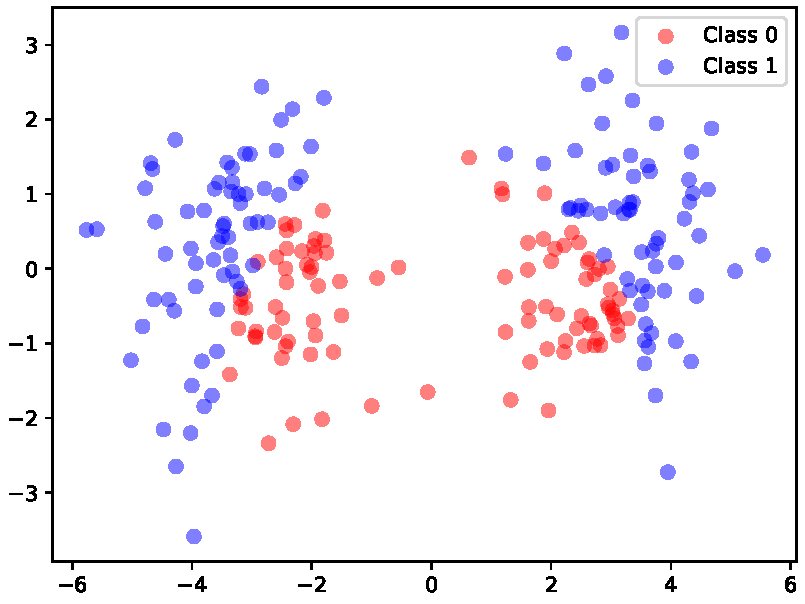
\includegraphics[scale=0.25]{chapter-2/images/data_xor.pdf}} & 
%         \subcaptionbox{...}{\includegraphics[scale=0.5]{chapter-2/images/MoE_toy.pdf}}\\
%     \end{tabular}
%     \caption[...]{...}
% \end{figure}

\begin{figure}[t]
\centering{
    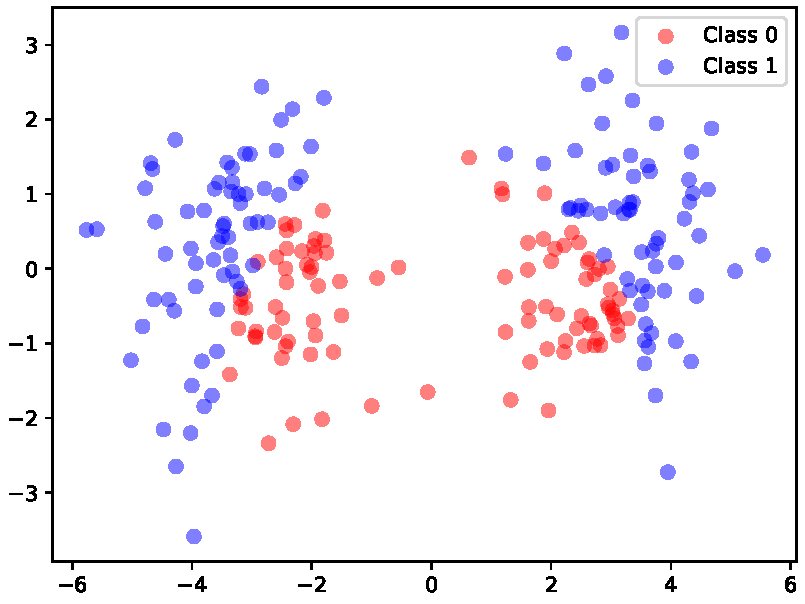
\includegraphics[scale=0.4]{chapter-2/images/data_xor.pdf}
    \caption{Synthetic data (best viewed in color) for the experiment with synthetic data in $\S~\ref{colsparseexp}$.}\label{fig:data-xor}
    }
\end{figure}

\begin{figure}[t]
\centering{
    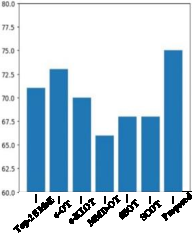
\includegraphics[width=0.35\columnwidth]{chapter-2/images/Toy-SMoE.pdf}
    \caption{Accuracies on the test split of synthetic data.}\label{fig:toy-tsne-acc}
    }
\end{figure}

\paragraph{Additional Details for Synthetic Data Experiment.}
Each of the experts is a 1-hidden-layer neural network with GELU as the activation function. The gating function is a single-layer neural network. We employ the Adam optimizer with a constant learning rate scheduler and train for 100 epochs.

In addition to the qualitative result discussed in Sec.~\ref{colsparseexp}, Fig.~\ref{tsne-data1-main}(d), we also report the test accuracy of our proposed approach, (vanilla) MoE, SCOT, and other SMoE baselines in which the (Top-$2$) gating function is based on entropy-regularized OT ($\epsilon$-OT) \citep{cuturi13a}, entropy-regularized KL-OT ($\epsilon$-KLOT) \citep{chizat17}, SSOT \citep{blondel18a}, and MMD-OT \citep{mmd-uot}. We observe that our method obtains the highest accuracy.

The randomly sampled validation split consists of $15\%$ instances. The regularization hyperparameter $\lambda$ for SCOT is chosen from $\{10^{-2}, 10^{-1}, 1, 10, 100\}$. For the proposed approach, $\lambda_1$ is chosen from $\{10^{2}, 10, 1\}$ and $\lambda_2$ is chosen from $\{10, 1\}$. For other baselines, the hyperparameters are chosen from the validation sets as described below.
(a) regularization hyperparameter for SSOT $\{10^{-2}, 10^{-1}, 1, 10 \}$, (b) for $\epsilon$-KLOT, marginal's regularization hyperparameter from $\{10^{-1}, 1, 10 \}$ and $\epsilon$ from $\{10^{-2}, 10^{-1}, 1, 10\}$, (c) regularization hyperparameter for entropic OT from $\{10^{-2}, 10^{-1}, 1, 10 \}$, and (d) the kernel-related hyperparameter and $\lambda_1$ for MMD-OT are chosen from the sets same as that for proposed Column-SparseOT method. 

The hyperparameters chosen for the proposed approach are IMQ-v2 kernel with $\sigma^2=100$ and regularization parameters $\lambda_1=100, \lambda_2=10$. The coefficient of regularization chosen for SCOT is $\lambda=10$.

\paragraph{Additional Details for CIFAR-10 Dataset Experiment.}
We follow \citet{chen2022towards} for the implementation of the base SMoE model. 
For the proposed method, we fix $\lambda_2=10$, the kernel function as IMQ-v2, and we set the kernel hyperparameter following the median-heuristics \citep{gretton12a}. The $\ell_2$-norm regularization hyperparameter $\lambda$ of SCOT and our $\lambda_1$ hyperparameter are chosen from $\{0.1, 10, 1000\}$.
The test data consists of 20000 examples, with 10000 examples each from CIFAR-10 and the CIFAR-10 rotated. 

The per-epoch computation time in seconds corresponding to Table~\ref{table-cifar} are 58.75s for (vanilla) MoE, 59.92s for SCOT, and  617.90s for our approach. 


\begin{table}[t]
\caption{Duality gap comparison for solving Problem (\ref{eqn:primal}) on varying the regularization hyperparameters. All values are rounded to 6 decimal places. The kernel used is IMQ. A lower duality gap is better.}
\label{table: DG-imq}
% \vskip 0.15in
\centering
\setlength{\tabcolsep}{4pt}
\begin{tabular}{ll|cc|cc}
\toprule
\multirow{2}{*}{$\lambda_1$} & \multirow{2}{*}{$\lambda_2$} & \multicolumn{2}{>{\columncolor{green!10}}c|}{Proposed solver} & \multicolumn{2}{c}{SCOT-based solver}\\
 &  & Primal optimal obj. & Duality Gap & Primal optimal obj. & Duality Gap \\ 
\midrule
0.1 & 0.1 & \cellcolor{green!10}{0.006073} &	\cellcolor{green!10}{$\mathbf{< 10^{-10}}$} & 0.006073 & 0.000020 \\
1 & 0.1 & \cellcolor{green!10}{0.040079}	& \cellcolor{green!10}{$\mathbf{0.000014}$} & 0.060187 	& 0.021549\\
10 & 0.1 & \cellcolor{green!10}{0.090064}	& \cellcolor{green!10}{$\mathbf{0.015801}$}	& 0.502088		& 0.418079 \\
0.1 & 1 & \cellcolor{green!10}{0.006073}	& \cellcolor{green!10}{$\mathbf{< 10^{-10}}$}	& 0.006073	& 0.000417 \\
1 & 1 & \cellcolor{green!10}{0.042633} &	\cellcolor{green!10}{$\mathbf{0.000012}$}	& 0.043374	& 0.001185 \\
10 & 1 & \cellcolor{green!10}{0.092715} & \cellcolor{green!10}{$\mathbf{0.001890}$}	& 0.095961 & 0.005033 \\ 
\bottomrule
\end{tabular}
% \vskip -0.1in
\end{table}

\subsection{Comparing Duality Gap}\label{app:dualitygap}
We detail adapting the SCOT-based solver for solving the dual (\ref{eqn:dual}) of the proposed primal problem (\ref{eqn:primal}).
Following \citet{liu2023sparsityconstrained}, we use the LBFGS optimizer from \texttt{scipy.optimize} and initialize the dual variables $\balpha, ~\bbeta$ as zero vectors of appropriate dimensions. Using the LBFGS optimizer requires one to pass a module that takes in inputs as the optimization variable ($\balpha, ~\bbeta$ in our case) and returns the objective value in (\ref{eqn:dual}) along with the expression for the gradient of the objective w.r.t. the optimization variables. The gradient of the dual objective w.r.t. $\balpha$ is $\bmu-\frac{\bG^{-1}_{11}\balpha}{2\lambda_1}-\mathbf{z}\bone$ and the gradient w.r.t. $\bbeta$ is $\bnu - \frac{\bG_{22}^{-1}\bbeta}{2\lambda_1}-\mathbf{z}^\top \bone$, where $\bz$ is the solution of the sparse projection problem (\ref{eqn:conjugate})  \citep{liu2023sparsityconstrained}. 

We set the maximum iteration limit for the APGD algorithm used in the proposed solver (Algorithm~\ref{alg:colsparseOT_dash}) as 1000. 
The results with the SCOT solver are also reported with 1000 as the maximum iteration (after confirming that a higher max-iter does not change the duality gap). 

Table~\ref{table: main-paper-DG-imq-v2} in the chapter shows duality gaps with the solvers employing IMQ-v2 kernel. 
The kernel hyperparameter is fixed according to the median heuristics \citep{gretton12a}, and the column-wise sparsity level is fixed as $K_2=4$. 
We observe that the proposed solver obtains better duality gaps across regularization hyperparameters and kernels. Additionally, Tables \ref{table: DG-imq} 
and \ref{table: DG-rbf} show the duality gaps associated with the proposed solver and the SCOT solver with RBF and IMQ kernels, respectively, and over different hyperparameter values. 


\begin{table}
\caption{Duality gap comparison for solving Problem (\ref{eqn:primal}) on varying the regularization hyperparameters. All values are rounded to 6 decimal places. The kernel used is RBF. A lower duality gap is better.}
\label{table: DG-rbf}
% \vskip 0.15in
\centering
\setlength{\tabcolsep}{4pt}
\begin{tabular}{ll|cc|cc}
\toprule
\multirow{2}{*}{$\lambda_1$} & \multirow{2}{*}{$\lambda_2$} & \multicolumn{2}{>{\columncolor{green!10}}c|}{Proposed solver} & \multicolumn{2}{c}{SCOT-based solver}\\
 &  & Primal optimal obj. & Duality Gap & Primal optimal obj. & Duality Gap \\ 
\midrule
0.1 & 0.1 & \cellcolor{green!10}{0.002000}	& \cellcolor{green!10}{$\mathbf{< 10^{-10}}$} & 0.002000	& $\mathbf{< 10^{-10}}$ \\
1 & 0.1 & \cellcolor{green!10}{0.019944}	& \cellcolor{green!10}{$\mathbf{< 10^{-10}}$} & 0.020003	& 0.000317\\
10 & 0.1 & \cellcolor{green!10}{0.094129}	& \cellcolor{green!10}{$\mathbf{0.057683	}$} & 0.174627 & 0.102349 \\
0.1 & 1 & \cellcolor{green!10}{0.002000}	&  \cellcolor{green!10}{$\mathbf{< 10^{-10}}$}	& 0.002000		& $\mathbf{< 10^{-10}}$ \\
1 & 1 & \cellcolor{green!10}{0.019953}	& \cellcolor{green!10}{$\mathbf{< 10^{-10}}$}	& 0.020218	& 0.000881\\
10 & 1 & \cellcolor{green!10}{0.094866}	& \cellcolor{green!10}{$\mathbf{0.008412}$}	& 0.155751	& 0.064417 \\ 
\bottomrule
\end{tabular}
% \vskip -0.1in
\end{table}


\begin{figure}[ht!]
  % \vskip 0.2in
  % \begin{center}
  \centering{
     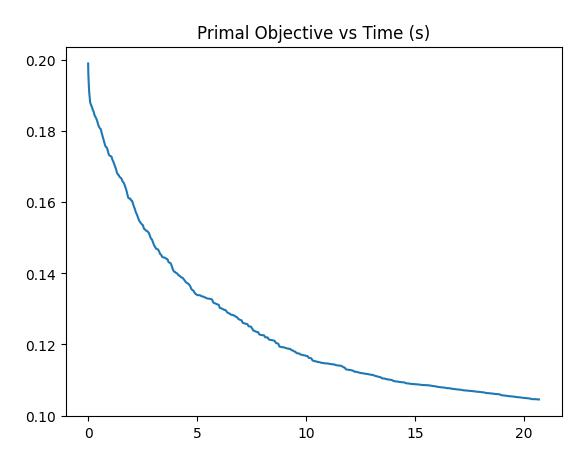
\includegraphics[scale=0.4]{chapter-2/images/primal_10.0_10.0_4.0.jpg}
     \caption{Primal objective vs Time (s) plot for solving the Column-SparseOT formulation using Algorithm~\ref{alg:colsparseOT_dash}. The computation is done on an Intel-i9 CPU.}\label{comp}
     }
 % \end{center}
 % \vskip -0.2in
 \end{figure}

\subsection{Optimization Curve}

Figure \ref{comp} shows the objective over time (s) plot (Intel-i9 CPU) for computing column-wise sparse transport plan using Algorithm \ref{alg:colsparseOT_dash}. The source and target measures are empirical measures over two randomly chosen 100-sized batches of CIFAR-10. The kernel used is RBF with median heuristics \citep{gretton12a}. The sparsity level $K_2$ is 4 and $\lambda_1=\lambda_2=10$. The computation is done on an Intel-i9 CPU.

 \begin{figure}[ht!]
    \centering
    \begin{tabular}{cccccc}
        \subcaptionbox{}{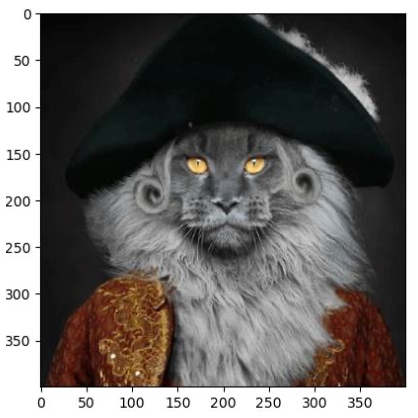
\includegraphics[scale=0.33]{chapter-2/images/Color-Transfer/ct1.pdf}} & 
        \subcaptionbox{}{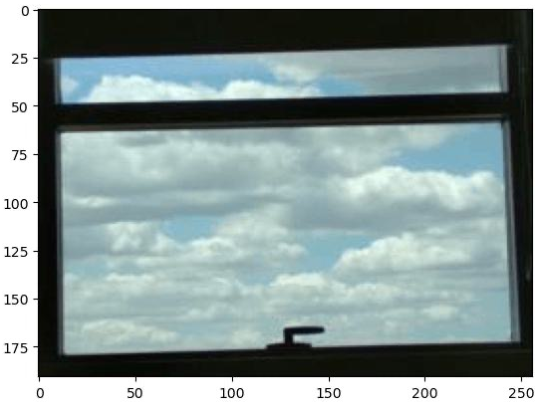
\includegraphics[scale=0.33]{chapter-2/images/Color-Transfer/ct2.pdf}} &
        \subcaptionbox{}{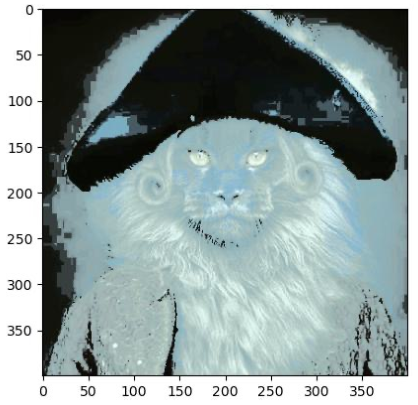
\includegraphics[scale=0.33]{chapter-2/images/Color-Transfer/ct3.pdf}} & 
        \subcaptionbox{}{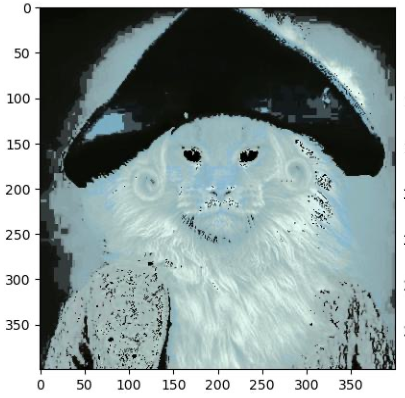
\includegraphics[scale=0.33]{chapter-2/images/Color-Transfer/ct4.pdf}} &
        \subcaptionbox{}{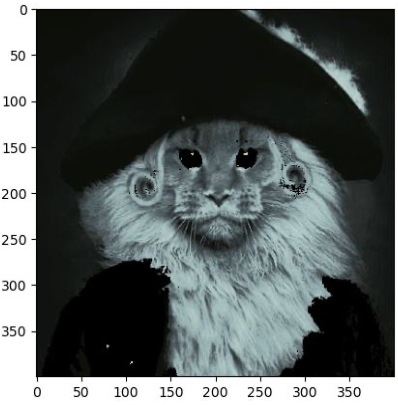
\includegraphics[scale=0.33]{chapter-2/images/Color-Transfer/ct5.pdf}} & 
        \subcaptionbox{}{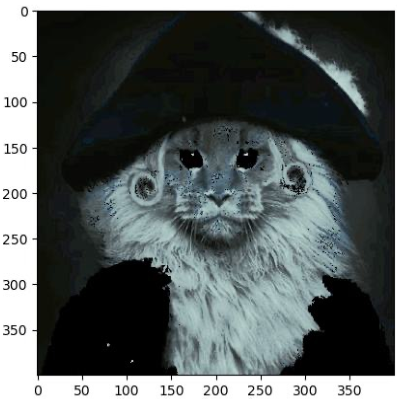
\includegraphics[scale=0.33]{chapter-2/images/Color-Transfer/ct6.pdf}}\\
    \end{tabular}
    \caption[Results on color transfer experiment.]{(Best viewed in color.) (a) Image 1 (b) Image 2. (c)-(f) show results (along with the level of sparsity) obtained by transferring the colors from Image 2 to Image 1: (c) OT ($99.22\%$) \cite{KatoroOT} (d) SSOT ($97.86\%$) \cite{blondel18a} (e) MMD-OT ($96.12\%$) \cite{mmd-uot} (f) Proposed General-SparseOT ($99.61\%$).}\label{color-cat}
 %     \label{color-cat}
 %     }
\end{figure}

\subsection{Color Transfer Experiment}
Following \citet{blondel18a}, we perform an experiment of OT-based color transfer. Figure~\ref{color-cat} shows the results with various methods and the sparsity level in the obtained transport map. The coefficient of $\ell_2$-norm regularization hyperparameter for SSOT is chosen 1 that obtained qualitatively best results. For the proposed method and for MMD-OT, we use RBF kernel with $\sigma^2=10^{-2}$ and $\lambda_1=0.1$.
\resumetoc